\section{Solving and Estimating the extended Model}

\subsection{Solution}

For this extended model I use the Double Deep-Q Network agent, since it was shown with the simpler model this model has comparable performance to the VFI implementation. The model is solved by running 3000 episodes. As was true for the simple model, the deep learning algorithm performs best if states are scaled mean 0 and a standard deviation of 1. This in practice by applying a transformer in my agent that can do a transformation of the states to be furthermore the transformer is capable of doing an inverse transformation. The rewards are also scaled, this slightly improves performance, but the primary reason is, that it helps track the learning. I scale the rewards to have a variance of about 1, and let them have the same mean conditional of the $\beta_L$  value! I train the algorithm for 3000 episodes, have the hyper parameters of the algorithm being: $\gamma=0.99$ representing the impatience of the agent. The agent is initialized with $\epsilon=1.0$ which decays by $0.9999$ for each step the agent performs. The learning rate is $\alpha=0.0005$. The size of the memory buffer is 1000000 rows, and I train with a batch size=64. I let the minimum exploration rate in training be $0.01$. I let the architecture of the network by identical to the simpler model: An Input layer of same size as the state space, 2 fully connected layers of size 256 with rectified linear units as activation functions, and an linear output layer of the same size as the action space. At the beginning of each episode a random $\beta_L \sim Uniform(0, 60)$, allowing the agent to step through an episode until terminal with given $\beta_L$. Finally the target network inherits the (XXX WEIGHTS) every $100$'th step. A score for every 50'th episode is run, taking the average of the previous 50 episodes. If the current iteration of the model beats the high score, the weights of the neural network is saved. The estimation and simulation is performed with the weights that yield the highest score for 50 consecutive episodes. 

\begin{figure}[ht]
    \centering
    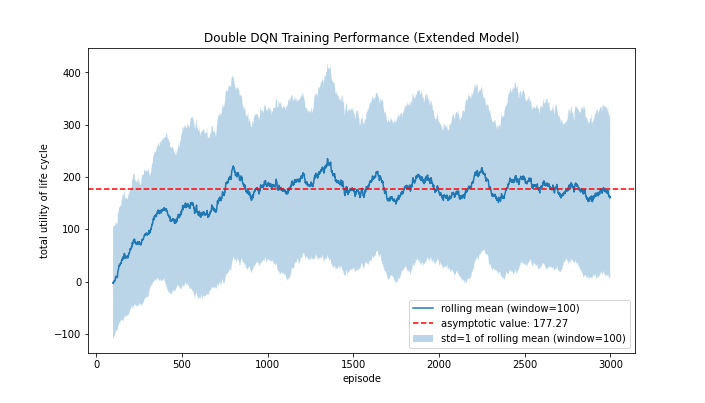
\includegraphics[scale=0.4]{figures/ddqn_extended_model_training_performance.png}
    \caption{Estimation of $\beta_L$ for extended model}
    \label{fig:training_extended}
\end{figure}

Looking to figure \ref{fig:training_extended} the agent clearly learns to navigate in the environment. After about 1000 episodes the agent seems to have learned to navigate the environment! The maximum score appears at around episode 1400, which is the weights used for estimation and simulations. The asymptotic training performance is about 180.


\subsection{Estimation}

Just as it was the case with the simpler model, only a single parameter $\beta_L$ needs to be estimated. Again, just as was the case before with the simpler model, I have extended the state space with $\beta_L$. I use a grid search in the range $\beta_L \in [0, 60]$, simulating $N=800$ observations, calculating the objective function. I use the same seed in each iteration of the optimization process. To address the short comings of the simple model i expand the objective function of the optimization problem. In the initial model to many women choose not to be part of the labour force yielding unrealistic results. Therefore the objective function now extends to two broad goals: Have the right number of women be out of the labour force (around15 \%) and let fit the curve of number of working hours for women. The first objective, \textit{objective 1}, is formulated as: 

\begin{equation}
    \text{objective 1} = \lsp\frac{\sum_{i=1}^{N} \sum_{t=1}^T \mathbf{1}\{H_{i,t} = 0\}}{ N \cdot (Q_{\max} - Q_{\min} )} - 15\% \rsp^2
\end{equation}

The second objective is formulated the same way as it was when first estimating the simpel model, which correspond the conditional expectation of supplied number of working hours conditional on the age and of being in the labour force $ \E[H \mid Q=q, H>0]$ Now the desired outcome is for this to be true for all ages from 18 to 60:


\begin{equation}
    \text{Objective 2} = \sum_{t=1}^{T} \lsp \frac{1}{\sum_{i=1}^{N} \mathbf{1}\{H_{i,t} > 0\}}\sum_{i=1}^N (H_{i,t})\rsp^2
\end{equation}

Now this description of the objectives can be translated into a more formal formulation. Considering this that there $\text{\# moments}  = 1 + (Q_{\max} - Q_{\min}) = 1 + 60 - 18 = 43$. Now the weighting of these moments would usually be done by some weight matrix $W$ in a formula looking like: $[\hat{m} - \tilde{m}]^{\top} W^{-1} [\hat{m} - \tilde{m}]$, where $\tilde{m}$ is a vector of empirical moments and $\hat{m}$ is a vector of simulated moments allowing for the methods of moments estimation. The choosing of the weight matrix is application specific. \textcite{eisenhauer_estimation_2015} suggests the choice in that setting should be the variance of empirical moments $\tilde{m}_j$, on the diagonal of the weight matrix (zeros else), letting the $j$'th moment correspond to the $j$'th weight. This is however not possible in this application, due to the fact, that I only have access to aggregated data from statistics Denmark. Instead i manually chooses scales such that \textit{objective 1} is equally weighted to \textit{objective 2}. This first and foremost requires a scaling of the moments. And second of all this requires a re weighting since there is 42 moments composing \textit{objective 2} and only a single moments composing \textit{objective 1}. Note here that since the distance between the empirical and the simulated moment is squared, the scaling must be performed before the squaring. Finally it should be noted that since the weight matrix is chosen as it is, a transformation can be performed such that instead of matrix product it can be considered a sum: $\sum_{j = 1}
^{43} ( \hat{m}_j - \tilde{m}_j )^2$. It is implied that $N$ agents is simulated conditional on a value of $\beta_L$. The objective function does in other words look as:

\begin{equation}
   \text{Objective}(\beta_L) =  \lsp 37 \cdot \lp\frac{\sum_{i=1}^{N} \sum_{t=1}^T \mathbf{1}\{H_{i,t} = 0\}}{ N \cdot (Q_{\max} - Q_{\min} )} - 15\% \rp \rsp^2 + \frac{1}{Q_{\max} - Q_{\min}}\sum_{t=1}^{T} \lsp \frac{1}{\sum_{i=1}^{N} \mathbf{1}\{H_{i,t} > 0\}}\sum_{i=1}^N (H_{i,t})\rsp^2
\end{equation}

\begin{figure}[ht]
    \centering
    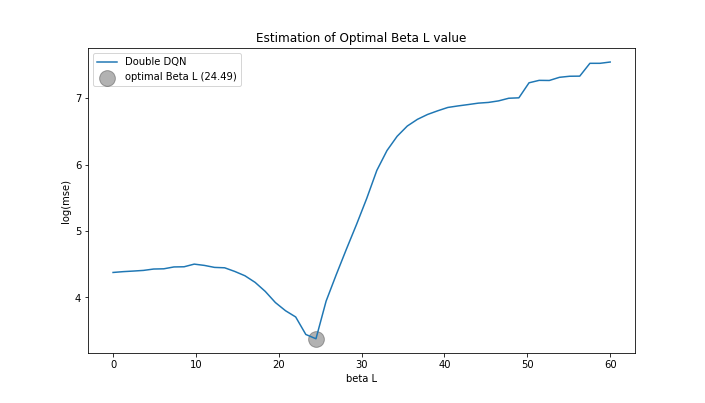
\includegraphics[scale=0.4]{figures/ddqn_extended_model_estimation_beta_L.png}
    \caption{Estimation of $\beta_L$ for extended model}
    \label{fig:estimation_extended}
\end{figure}

The estimated value of $\beta_L = 24.49$. Figure \ref{fig:estimation_extended} shows the grid search, and finds that optimization problem, does seem to have a fairly unique minima at $\beta_L = 24.49$, suggesting that the range of the grid is adequate for the estimation problem. I take the $\log (\cdot)$ of the mean squared error to better represent it in figure XXX, allowing for not showing the less extreme tails.